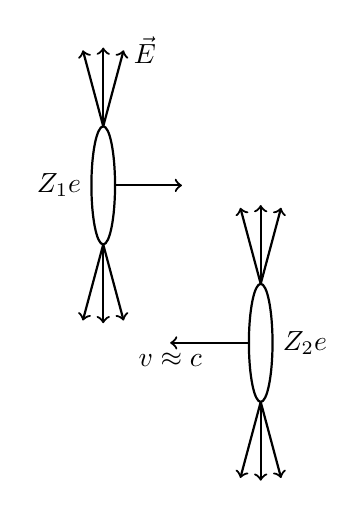
\begin{tikzpicture}[thick]
	\draw(-2,2) ellipse (0.15 and 0.75);
	\draw(0,0) ellipse (0.15 and 0.75);
	\node[left] (z1) at (-2.15,2) {$Z_1e$};
	\node[right] (z2) at (0.15,0) {$Z_2 e$};

	\draw[->](-2,2.75) -- (-2,3.75);
	\draw[->, rotate around={15:(-2,2.75)}](-2,2.75) -- (-2,3.75);
	\draw[->, rotate around={-15:(-2,2.75)}](-2,2.75) -- (-2,3.75)
		node[right]{$\vec{E}$};

	\draw[->](-2,1.25) -- (-2,0.25);
	\draw[->, rotate around={15:(-2,1.25)}](-2,1.25) -- (-2,0.25);
	\draw[->, rotate around={-15:(-2,1.25)}](-2,1.25) -- (-2,0.25);

	\draw[->](0,0.75) -- (0,1.75);
	\draw[->, rotate around={15:(0,0.75)}](0,0.75) -- (0,1.75);
	\draw[thick, ->, rotate around={-15:(0,0.75)}](0,0.75) -- (0,1.75);

	\draw[->](0,-0.75) -- (0,-1.75);
	\draw[->, rotate around={15:(0,-0.75)}](0,-0.75) -- (0,-1.75);
	\draw[->, rotate around={-15:(0,-0.75)}](0,-0.75) -- (0,-1.75);

	\draw[->](-1.85,2) -- (-1,2);
	\draw[->](-0.15,0) -- (-1.15,0) node[below]{$v \approx c$};
\end{tikzpicture}

